\section{Direct Prediction: BrainScore and BehavScore}
\label{app:direct}

The original benchmark scores models by direct prediction: a ridge encoder maps a model's hidden states to each response (embedding track), and a mixed-effects regression measures the held-out gain from its surprisal (surprisal track). Unlike the RDM regression, both fit a learned mapping from the model to the data. This appendix gives the design, the Pareto fronts and the matched-scale analysis of the two tracks, each at the last layer and at the best layer of every model.

\subsection{Design}
\label{sec:design-tracks}

\paragraph{Surprisal track.}
Surprisal is the negative log probability of a word, summed over its subword tokens. For each dataset we fit a linear mixed-effects model with dataset-specific nuisance predictors (word length and frequency for reading data, plus the covariates required by each neural recording design) and compare it with the model that adds the current word's surprisal and, where specified, the previous word's surprisal as a spillover term. Random-effect structures are dataset-specific (Appendix~\ref{app:lme-formulas}). The score is the improvement in held-out log likelihood per test observation,
\begin{equation}
\Delta\ell_{\mathrm{LME}}=\frac{\ell_{\mathrm{full}}^{\mathrm{test}}-\ell_{\mathrm{base}}^{\mathrm{test}}}{n_{\mathrm{test}}},
\label{eq:dll-lme}
\end{equation}
divided by a split-half $\Delta\ell$ reference built from the human data \citep{timkey2026dissociation}. The \emph{last-layer} score uses the model's output distribution. The \emph{best-layer} score reads surprisal out of every layer through the output head (logit lens) and keeps the layer with the highest \emph{training} $\Delta\ell$, so the scored folds play no part in the choice.

\paragraph{Scores and regression.}
A model's \emph{BrainScore} is the median of its normalized scores over the neural dataset units and its \emph{BehavScore} the median over the 16 behavioral measures. The matched-scale regression is Equation~\ref{eq:group}, fitted separately per domain with a dataset-unit random intercept, on all 118 models. The embedding track uses all 11 neural units (1,870 behavioral and 1,290 neural rows). The surprisal track leaves out the four neural datasets whose $\Delta\ell$ references are unusable, because models exceed them or most scores are negative (Broderick, Federmeier 2007, Hubbard 2019 and Pereira), giving 1,870 behavioral and 818 neural rows.

\subsection{Embedding track}
\label{app:direct-embedding}

\begin{figure}[h]
\centering
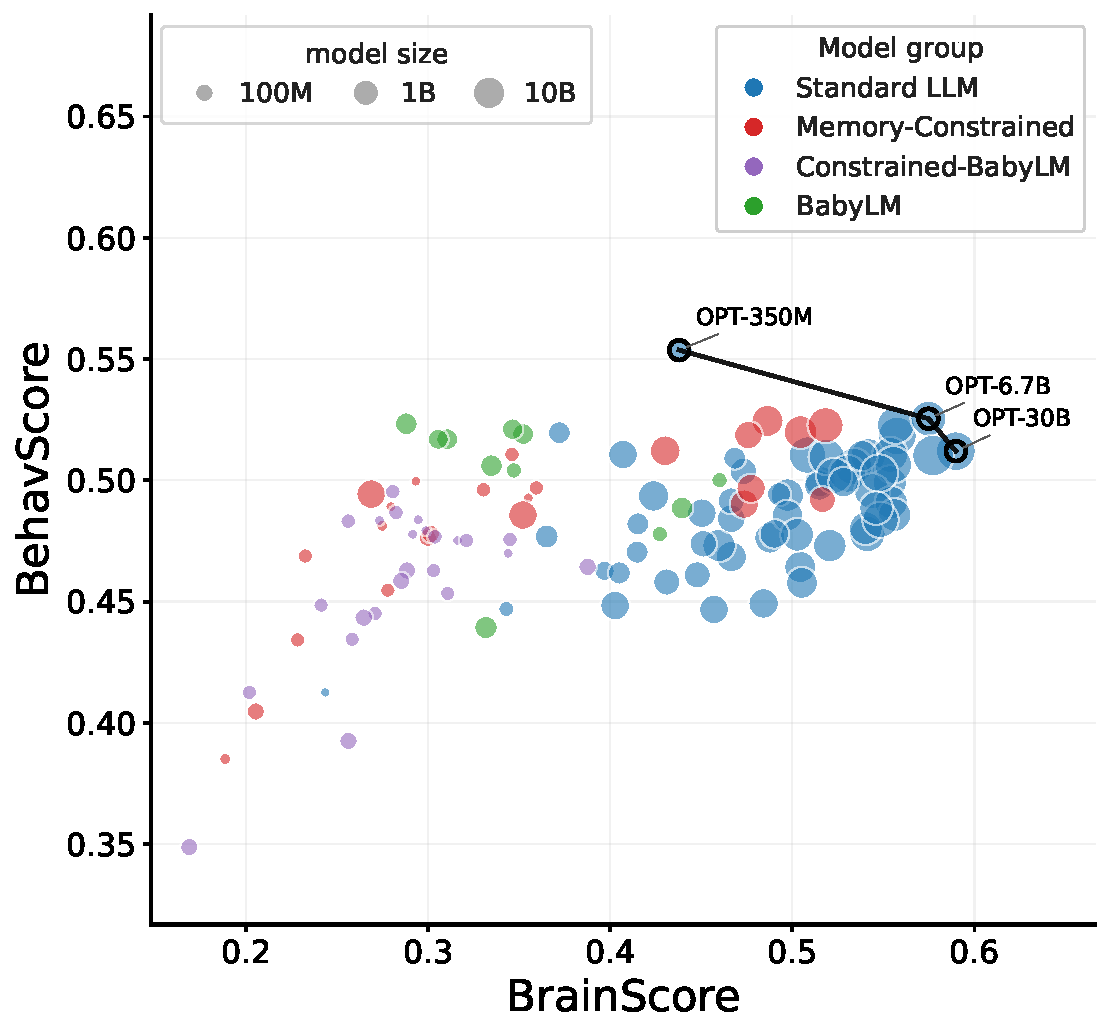
\includegraphics[width=.49\linewidth]{figures/direct_embedding_lastlayer_pareto.pdf}\hfill
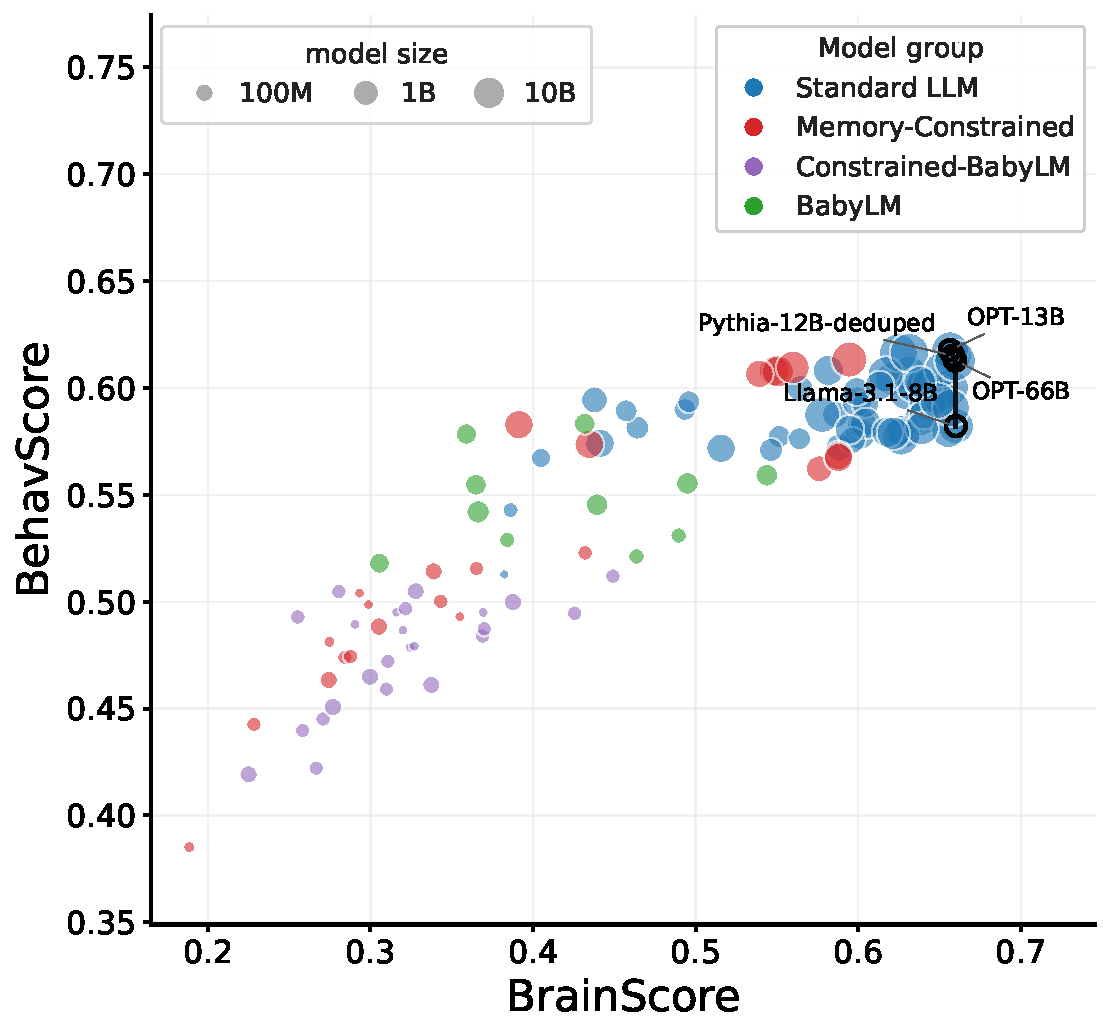
\includegraphics[width=.49\linewidth]{figures/direct_embedding_bestlayer_pareto.pdf}
\caption{BrainScore against BehavScore for the embedding track (ridge encoding, Pearson $r$ divided by the correlation ceiling), last layer (left) and best layer (right); 118 models. Layout as in Figure~\ref{fig:pareto}.}
\label{fig:direct-embedding}
\end{figure}

\begin{table}[t]
\centering
\small
\setlength{\tabcolsep}{4pt}
\caption{Matched-scale regression on the direct embedding scores (ridge encoding / decoding, Pearson $r$ divided by the correlation ceiling), fitted separately per domain with a dataset random intercept (REML, Wald tests); 118 models, 1,870 behavioral and 1,290 neural rows.}
\label{tab:direct-embedding}
\resizebox{\linewidth}{!}{%
\begin{tabular}{lcccc}
\toprule
 & \multicolumn{2}{c}{BehavScore} & \multicolumn{2}{c}{BrainScore} \\
\cmidrule(lr){2-3}\cmidrule(lr){4-5}
 & Last layer & Best layer & Last layer & Best layer \\
\midrule
Memory constraint $\beta_M$ & $+0.015^{***}$ (0.003) & $-0.023^{***}$ (0.002) & $-0.023^{**}$ (0.008) & $-0.055^{***}$ (0.007) \\
Data constraint $\beta_D$ & $+0.033^{***}$ (0.003) & $-0.002$ (0.003) & $-0.001$ (0.010) & $-0.030^{***}$ (0.009) \\
Interaction $\beta_{MD}$ & $-0.041^{***}$ (0.004) & $-0.024^{***}$ (0.004) & $-0.005$ (0.012) & $+0.018$ (0.011) \\
$\log_{10}$ parameters $\beta_S$ & $+0.012^{***}$ (0.001) & $+0.018^{***}$ (0.001) & $+0.048^{***}$ (0.004) & $+0.053^{***}$ (0.004) \\
$\log_{10}$ perplexity $\beta_P$ & $-0.005^{***}$ (0.001) & $-0.014^{***}$ (0.001) & $-0.005$ (0.004) & $-0.016^{***}$ (0.004) \\
\bottomrule
\end{tabular}}
\par\smallskip{\footnotesize Coefficient (SE); reference = Standard LLM. $^{*}p<.05$, $^{**}p<.01$, $^{***}p<.001$.}
\end{table}


At the last layer, the front consists of three OPT models, from OPT-350M (BehavScore .554) through OPT-6.7B to OPT-30B (BrainScore .590). BabyLM models have the highest median BehavScore (.506, against .467--.492 for the other groups), while Standard LLMs have the highest median BrainScore (.503, against .287--.346). At the best layer the front is made of four large Standard LLMs (OPT-13B, Pythia-12B, OPT-66B and Llama-3.1-8B) whose scores differ by less than .04 on either axis, so there is no trade-off between groups, and Standard LLMs have the highest medians on both (.591 and .621).

At matched size and perplexity (Table~\ref{tab:direct-embedding}), the last-layer scores show the dissociation of the main analysis for the memory constraint: it is associated with a higher BehavScore ($+.015$, $p<.001$) and a lower BrainScore ($-.023$, $p=.003$). The data constraint is associated with a higher BehavScore ($+.033$, $p<.001$) and not with BrainScore, and the interaction is negative for behavior ($-.041$). At the best layer, the memory constraint is associated with lower scores in both domains (behavior $-.023$, brain $-.055$, both $p<.001$) and the data constraint with a lower BrainScore only ($-.030$, $p<.001$). Size is positive in both domains at both layers, so the ridge track shows no size dissociation.

\subsection{Surprisal track}
\label{app:direct-surprisal}

\begin{figure}[h]
\centering
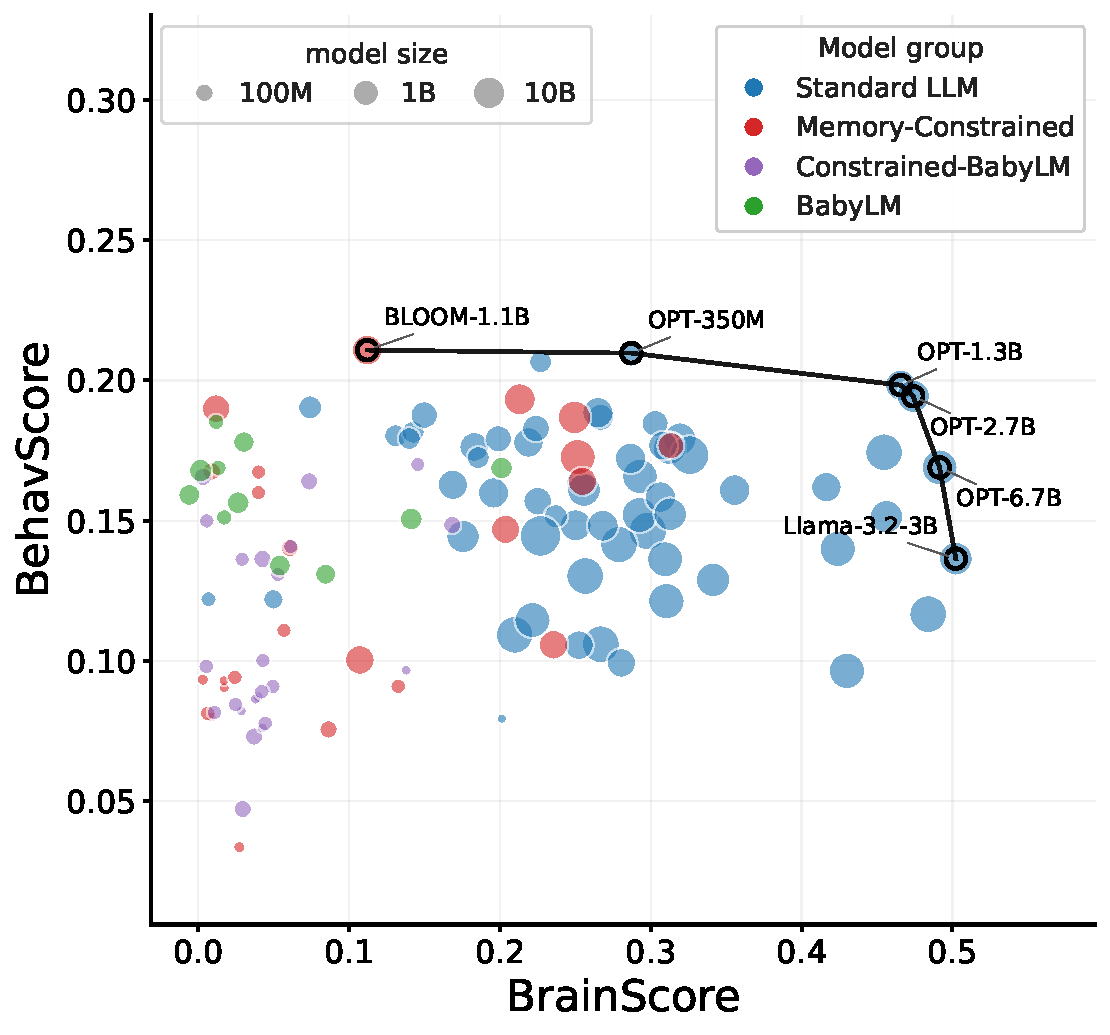
\includegraphics[width=.49\linewidth]{figures/direct_surprisal_lastlayer_pareto.pdf}\hfill
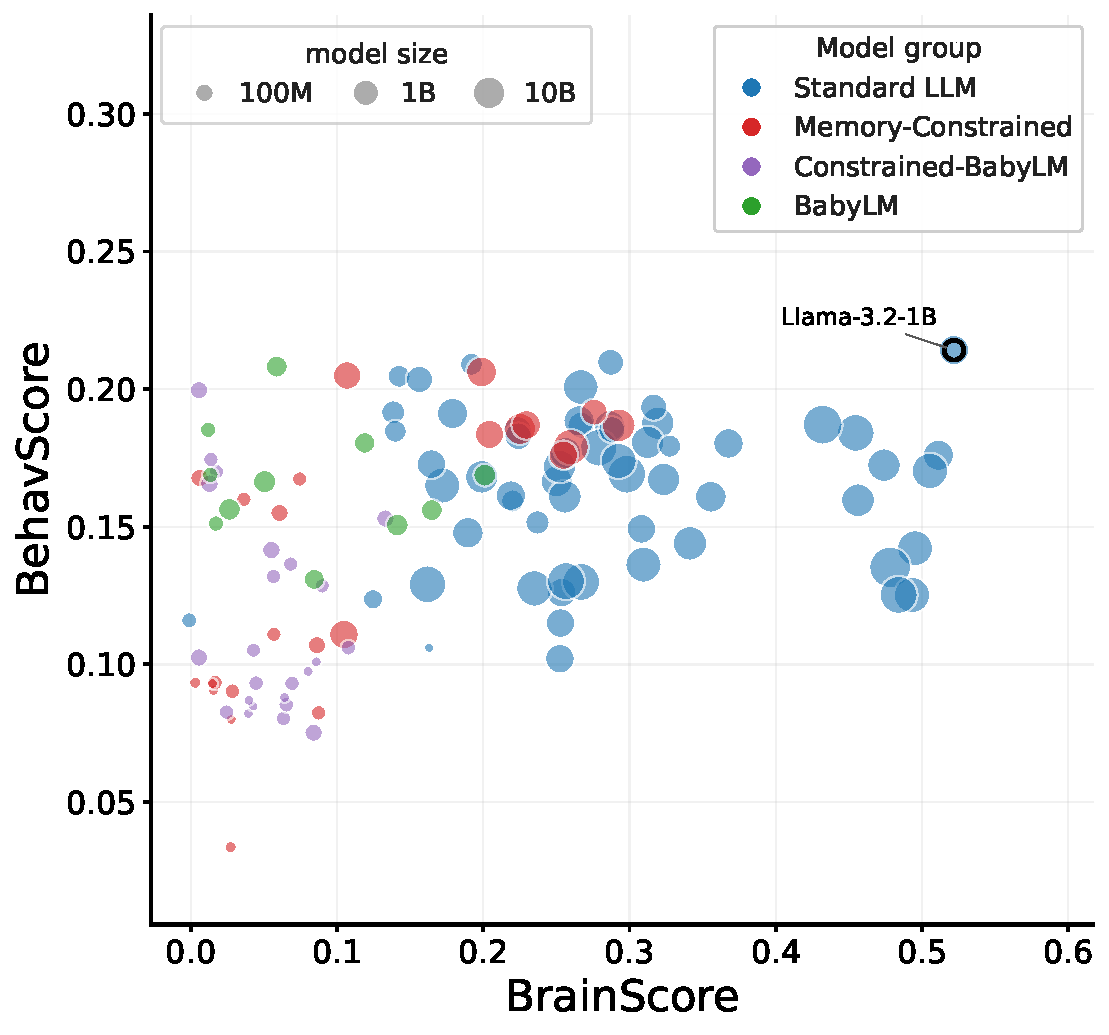
\includegraphics[width=.49\linewidth]{figures/direct_surprisal_bestlayer_pareto.pdf}
\caption{BrainScore against BehavScore for the surprisal track (pooled LME, $\Delta\ell$ divided by the $\Delta\ell$ reference), last layer (left) and best layer, chosen on the training $\Delta\ell$ (right); 118 models. Layout as in Figure~\ref{fig:pareto}.}
\label{fig:direct-surprisal}
\end{figure}

\begin{table}[t]
\centering
\small
\setlength{\tabcolsep}{4pt}
\caption{Matched-scale regression on the direct surprisal scores (pooled LME, held-out $\Delta$log-likelihood divided by the $\Delta$log-likelihood ceiling; best layer chosen on the training $\Delta$log-likelihood), fitted separately per domain with a dataset random intercept (REML, Wald tests); 118 models, 1,870 behavioral and 818 neural rows (Broderick, Federmeier 2007, Hubbard 2019 and Pereira are left out because their $\Delta$log-likelihood references are unusable).}
\label{tab:direct-surprisal}
\resizebox{\linewidth}{!}{%
\begin{tabular}{lcccc}
\toprule
 & \multicolumn{2}{c}{BehavScore} & \multicolumn{2}{c}{BrainScore} \\
\cmidrule(lr){2-3}\cmidrule(lr){4-5}
 & Last layer & Best layer & Last layer & Best layer \\
\midrule
Memory constraint $\beta_M$ & $+0.004$ (0.005) & $+0.007$ (0.006) & $-0.008$ (0.015) & $+0.010$ (0.017) \\
Data constraint $\beta_D$ & $+0.032^{***}$ (0.007) & $+0.034^{***}$ (0.007) & $-0.026$ (0.019) & $-0.014$ (0.021) \\
Interaction $\beta_{MD}$ & $-0.039^{***}$ (0.008) & $-0.036^{***}$ (0.009) & $+0.038$ (0.022) & $+0.017$ (0.025) \\
$\log_{10}$ parameters $\beta_S$ & $-0.022^{***}$ (0.003) & $-0.011^{**}$ (0.003) & $+0.029^{***}$ (0.009) & $+0.035^{***}$ (0.010) \\
$\log_{10}$ perplexity $\beta_P$ & $-0.035^{***}$ (0.003) & $-0.035^{***}$ (0.003) & $-0.015$ (0.007) & $-0.007$ (0.009) \\
\bottomrule
\end{tabular}}
\par\smallskip{\footnotesize Coefficient (SE); reference = Standard LLM. $^{*}p<.05$, $^{**}p<.01$, $^{***}p<.001$.}
\end{table}


At the last layer, the front runs from BLOOM-1.1B (Memory-Constrained; BehavScore .211) through OPT models to Llama-3.2-3B (BrainScore .502). Standard LLMs have the highest median BrainScore (.267, against .026--.059), while BabyLM and Standard LLMs have similar median BehavScores (.159 and .161). At the best layer, a single Standard LLM, Llama-3.2-1B, leads on both scores.

At matched size and perplexity (Table~\ref{tab:direct-surprisal}), the data constraint is associated with a higher BehavScore at both layers ($+.032$ and $+.034$, $p<.001$), the memory constraint is not reliable ($p>.20$), and the interaction is negative ($-.039$ and $-.036$). No constraint is associated with BrainScore. Size shows the dissociation of the main analysis: larger models have a lower BehavScore ($-.022$ last, $-.011$ best) and a higher BrainScore ($+.029$ and $+.035$, $p\leq.001$).

\subsection{Comparison with the representational evaluation}
\label{app:direct-summary}

The data constraint is associated with higher behavioral scores in the RDM regression and in both direct tracks at the last layer. The brain penalty of the constraints and the size dissociation depend on the evaluation. The memory penalty on the brain appears in the ridge track and in the two-dataset RDM regression, is not reliable in the all-dataset RDM regression ($p=.10$), and is absent in the surprisal track. The size dissociation appears in the RDM regression and in the surprisal track, but not in the ridge track, where larger models score higher in both domains. With best-layer selection, the ridge track no longer shows a trade-off between groups: large Standard LLMs lead on both scores.
